%
% chapter.tex -- Kapitel über die Geometrie von Wavelets
%
% (c) 2019 Prof Dr Andreas Müller
%
\chapter{Sampling und Geometrie
\label{chapter:geometrie}}
\lhead{Sampling und Geometrie}
In der Einleitung haben wir gesehen, dass wir eine Technik brauchen,
Signale miteinander zu vergleichen.
In diesem Kapitel bauen wir eine solche Technik auf und entwickeln
auch eine geometrische Sprache dafür.
Diese hilft uns, die Analyse- und Synthese-Formeln auf eine Art zu formulieren,
die uns erlaubt die Gemeinsamkeiten besser zu verstehen unabhängig von
der konkreten Form der verwendeten Vergleichsfunktionen.
Es stellt sich heraus, dass das Konzept des Skalarproduktes aus der
Vektorgeometrie genau die richtige Intuition liefert.
Wir verallgemeinern diese Ideen auf Mengen von Funktionen.
Wir erhalten so das Konzept des Hilbert-Raumes, der unendlichdimensionalen 
Verallgemeinerung des Vektorraumes mit einem Skalarprodukt.

In diesem Kapitel stellen wir im ersten Abschnitt den Zusammenhang
zwischen Signalvergleich und Skalarprodukt her.
Im zweiten Abschnitt formulieren wir den Begriff des Hilbertraumes
und die grundlegendsten Eigenschaften.
Die Aufgabe der Rekonstruktion eines Signals aus den Fourierkoeffizienten
verallgemeinern wir in Abschnitt~\ref{section:rekonstruktion} auf beliebige
Hilberräume.

In der linearen Algebra lernt man, in einem Vektorraum Problem mit einer
Basis, wenn möglich mit einer orthonormierten Basis zu lösen.
In der Praxis der Signalverarbeitung ist dies zu einschränkend.
Dieses Phänomen findet man bereits in der elementaren Geometrie.
Bienenwaben in der Ebene können natürlich mit einem rechtwinkligen
Koordinatensystem beschrieben werden, doch ein Koordinatensystem mit
Achsen, die einen Winkel von $60^\circ$ einschliessen, ist besser an
das Problem angepasst.
Genausogut ist jedoch auch ein Koordinatensystem  mit Achsen, die einen
Winkel von $120^\circ$ einschliessen.
Fügt man eine dritte Achse hinzu, kann man sich diesem Dilemma entziehen,
dafür führt man Redundanz ein.
Daher untersuchen wir in Abschnitt~4, wie man den Begriff der Basis
zu einem Begriff eines Frames erweitern kann, welches zwar redundant
ist, aber dank zusätzlicher Symmetrien besser geeignet ist.

%
% vergleich.tex -- vergleich von signalen
%
% (c) 2019 Prof Dr Andreas Müller, Hochschule Rapperswil
%
\section{Vergleich von Signalen und Vektorgeometrie
\label{section:vergleich}}
\rhead{Vergleich von Signalen und Vektorgeometrie}
In diesem Abschnitt suchen wir eine geometrische Sprache für das
Problem, zwei Signale zu vergleichen und ein Signal aus geeigneten
Vergleichssignalen zusammenzusetzen.

\subsection{Vergleich von Signalen}
Beginnend mit Binärsignalen entwickeln wir ein anschauliches Mass für die
``Ähnlichkeit'' von zwei Signalen.

\subsubsection{Binärsignale}
Wir beginnen unsere Betrachtungen mit zwei diskrete Signale mit Werten $\pm 1$:
\begin{align*}
&x_1,x_2,x_3,\dots,x_N &&\in \{\pm 1\},
\\
&y_1,y_2,y_3,\dots,y_N &&\in \{\pm 1\},
\end{align*}
und versuchen eine Masszahl für die Ähnlichkeit dieser beiden
Zahlfolgen zu entwickeln.

Die Masszahl muss umso grösser sein, je öfter die Folgenglieder
übereinstimmen, also $x_k=y_k$.
Indizes $k$, für die die Folgenglieder entgegengesetzt sind, also
$x_k\ne y_k$, müssen dagegen abgezogen werden.
Eine mögliche Masszahl ist daher 
\[
\sum_{k=1}^N x_ky_k.
\]
Sind die beiden Folgen identisch, wird die Summe $N$.
Sind die beiden Folgen genau entgegengesetzt, also $x_k=-y_k$, dann ist
sie $-N$.
Die Masszahl ist damit abhängig von der Anzahl der Datenpunkte.
Damit wird es nicht gut möglich, Funktionsvergleiche über verschieden
lange Datensätze miteinander zu vergleichen.
Das Problem wird gelöst, indem man durch $N$ teilt und als Masszahl
\[
p=\frac{1}{N} \sum_{k=1}^N x_ky_k
\]
verwendet.
Die Extremwerte werden jetzt $p=1$ für übereinstimmende Signale und
$p=-1$ für entgegengesetzte Signale.

Wenn die beiden Folgen nichts mitenander zu tun haben, dann erwarten
wir, dass $x_k$ und $y_k$ jeweils etwa in der Hälfte der Fälle
entgegengesetztes Vorzeichen haben werden, und gleiches in allen
anderen.
Dies führt auf $p=0$.
Die Zahl $p$ könnte also als Mass dafür dienen, wie ähnlich die beiden Signale
sind.

Dies ist allerdings nicht ganz realistisch.
Warum sollten die Werte $+1$ und $-1$ gleich häufig sein?
Man könnte dies korrigieren, indem man den mittleren Wert beider Folgen
subtrahiert.
So erhält man die Kovarianz
\begin{equation}
\operatorname{cov}(x_k,y_k)
=
\frac1{N} \sum_{k=1}^N x_ky_k
-
\frac1{N} \sum_{k=1}^N x_k
\cdot
\frac1{N} \sum_{k=1}^N y_k.
\label{geometrie:cov}
\end{equation}
Die Kovarianz verschwindet genau dann, wenn beiden Signale $x_k$ und $y_k$
völlig unkorreliert sind.
Offenbar reicht es auch vollständig aus, wenn nur eines der Signale
im Mittel den Wert $0$ hat, dann verschwindet der zweite Term
in~\eqref{geometrie:cov}.

\subsubsection{Reellwertige Signale}
\begin{figure}
\centering
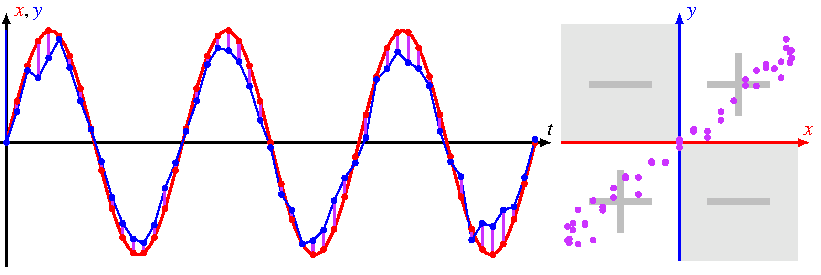
\includegraphics[width=\hsize]{chapters/1-geometrie/images/sinsin.pdf}
\caption{Vergleich eines Sinus-Signals $\color{red}x(t)$ mit einem
verrauschen Sinus-Signal $\color{blue}y(t)$.
Die Punkte $({\color{red}x(t)},{\color{blue}y(t)})$ befinden sich
hauptsächlich im ersten und dritten Quadranten.
\label{geometrie:kovarianz:sinsin:image}}
\end{figure}
\begin{figure}
\centering
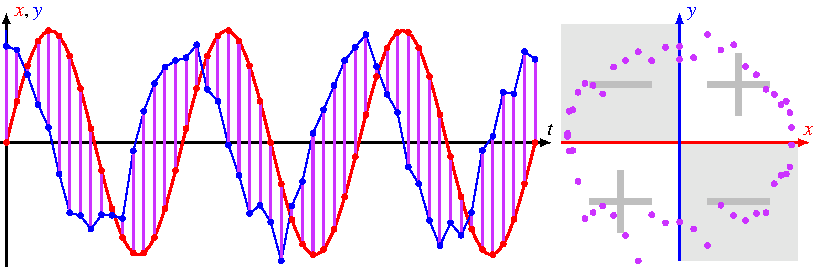
\includegraphics[width=\hsize]{chapters/1-geometrie/images/sincos.pdf}
\caption{Vergleich eines Sinus-Signals $\color{red}x(t)$ mit einem
verrauschen Kosinus-Signal $\color{blue}y(t)$.
Die Punkte $({\color{red}x(t)},{\color{blue}y(t)})$ befinden sich
in ungefähr gleicher Zahl in allen vier Quadranten, die Kovarianz
wird klein sein.
\label{geometrie:kovarianz:sincos:image}}
\end{figure}
\begin{figure}
\centering
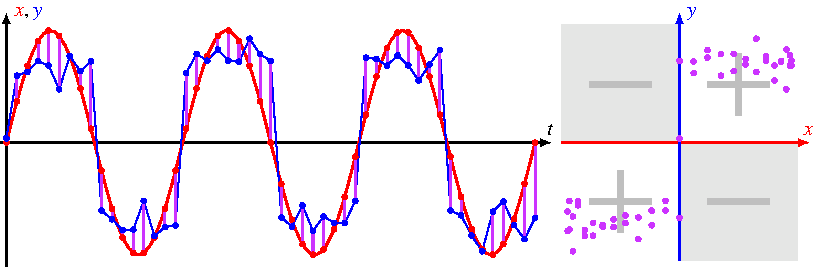
\includegraphics[width=\hsize]{chapters/1-geometrie/images/sinrect.pdf}
\caption{Vergleich eines Sinus-Signals $\color{red}x(t)$ mit einem
verrauschen Rechteck-Signal $\color{blue}y(t)$.
Die Punkte $({\color{red}x(t)},{\color{blue}y(t)})$ befinden sich
hauptsächlich im ersten und dritten Quadranten.
\label{geometrie:kovarianz:sinrect:image}}
\end{figure}
\begin{figure}
\centering
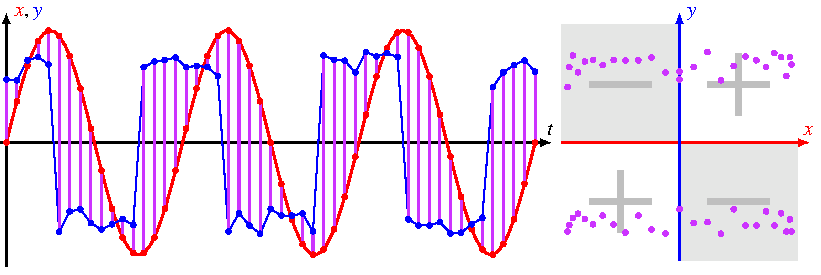
\includegraphics[width=\hsize]{chapters/1-geometrie/images/cosrect.pdf}
\caption{Vergleich eines Sinus-Signals $\color{red}x(t)$ mit einem
verrauschen und phasenverschobenen Rechteck-Signal $\color{blue}y(t)$.
Die Punkte $({\color{red}x(t)},{\color{blue}y(t)})$ befinden sich
in ungefähr gleicher Zahl in allen vier Quadranten, die Kovarianz
wird klein sein.
\label{geometrie:kovarianz:cosrect:image}}
\end{figure}
\begin{figure}
\centering
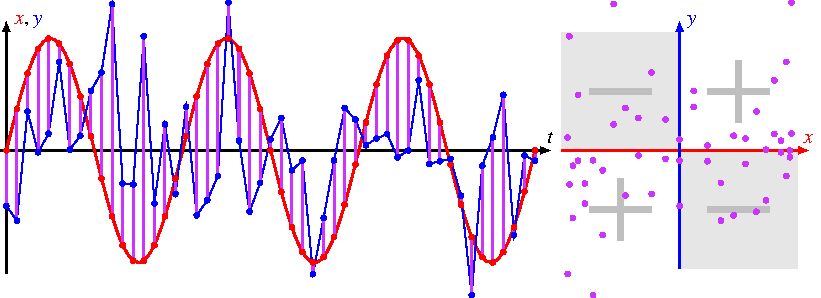
\includegraphics[width=\hsize]{chapters/1-geometrie/images/sinrand.pdf}
\caption{Vergleich eines Sinus-Signals $\color{red}x(t)$ mit einem
weissen Rausch-Signal $\color{blue}y(t)$ (normalverteilte Zufallswerte
mit Erwartungswert $0$).
Die Punkte $({\color{red}x(t)},{\color{blue}y(t)})$ befinden sich
in ungefähr gleicher Zahl in allen vier Quadranten, die Kovarianz
wird klein sein.
\label{geometrie:kovarianz:sinrand:image}}
\end{figure}


Binäre Signale sind nicht allzu realistisch, wir möchten daher zwei
beliebige rellwertige Signale vergleichen.
Die früher verwendete Summe der Produkte der Signalwerte wird grösser,
wenn die Signalwerte grösser werden, sie ist also nicht geeignet als
absolutes Mass für die Ähnlichkeit zweier Funktionen.
Wir müssen daher mit einem Faktor korrigieren, der die ungefähre
Grösse der Absolutbeträge des Signals wiedergibt.
\[
\frac1{N}
\sum_{k=1}^N x_k^2
\qquad\text{bzw.}\qquad
\frac1{N}
\sum_{k=1}^N y_k^2
\]
verwenden.
Diese haben allerdings die falsche Masseinheit, nämlich die des
Quadrates des Signals, wir müssen also ihre Quadratwurzel verwenden.
Für Signale mit Mittelwert $0$ führt dies auf
\[
\frac{
\frac{1}{N}\sum_{k=1}^N x_ky_k
}{
\sqrt{\frac{1}{N}\sum_{k=1}^N x_k^2}
\sqrt{\frac{1}{N}\sum_{k=1}^N y_k^2}
}
\qquad\text{oder}\qquad
r
=
\frac{\operatorname{cov}(x_k,y_k)}{\sqrt{\operatorname{var}(x_k)}\sqrt{\operatorname{var}(y_k)}}
\]
Die Grösse $r$ ist auch bekannt als der Korrelationskoeffizient.

In den Abbildung~\ref{geometrie:kovarianz:sinsin:image} bis
\ref{geometrie:kovarianz:sinrand:image} wird ein Sinus-Signal
mit Werten $x(t)=sin t$ abgetastet und verglichen mit
einer Reihen anderer Signale,
die alle ebenfalls den Mittelwert $0$ haben.
Wir wollen beurteilen, wie gut die Summe
\[
\frac{1}{N}\sum_{k=1}^N x_ky_k
\]
wiedergibt, ob die Funktionen etwas miteinander zu tun haben.
Dazu wird im linken Teil der Abbildung jeweils das Sinus-Signal
$x(t)$ rot eingezeichnet und das damit zu vergleichende Signal $y(t)$
blau.
Der Unterschiede zwischen den beiden Werten wird durch einen 
violetten Balken eingezeichnet.

Im rechten Teil der Abbildung wird dann für jeden Zeitpunkt
das Wertepaar $(x(t),y(t))$ als violetter Punkt eingetragen.
Punkte im ersten und dritten Quadranten führen auf einen positiven
Summanden in der Summe, Punkte im zweiten und vierten Quadranten
führen auf einen negativen Beitrag.
Die Summe wird also besonders gross, wenn die violetten Punkte vor
Allem im ersten und dritten Quadranten liegen, und besonders negativ,
wenn sie vor Allem im zweiten und vierten Quadranten liegen.

Liegen die violetten Punkte in allen Quadranten gleichmässig, ist
davon auszugehen, dass sich die positiven und negativen Werte des
Produktes im Mittel wegheben werden, dass also die Summe der
Produkte nur einen kleinen Werte haben wird.

Die Abbildungen~\ref{geometrie:kovarianz:sinsin:image} und
\ref{geometrie:kovarianz:sinrect:image} zeigen den Vergleich
des Sinus-Signals mit einer verrauschen Version eines Sinus-Signals
bzw.~eines Rechteck-Signals $\operatorname{sign}(\sin(t))$.
In beiden Fällen liegen die violetten Punkte vorzugsweise im ersten
und dritten Quadranten, 

In den anderen Abbildungen
wird das Sinus-Signal der Reihe nach mit einem verrauschten
Kosinus-Signal (Abbildung~\ref{geometrie:kovarianz:sincos:image}),
einem phasenverschobenen verrauschten Rechtecksignal
(Abbildung~\ref{geometrie:kovarianz:cosrect:image})
und mit einem reinen weissen Rauschen
(Abbildung~\ref{geometrie:kovarianz:sinrand:image})
verglichen.
In diesen Fällen verteilen sich die violetten Punkte gleichmässig
über alle vier Quadranten, man erwartet also einen kleinen Wert
der Summe, was eine geringe Ähnlichkeit der blauen Signale mit dem
Sinus-Signal ausdrückt.

%Doch auch dies kann nicht ganz richtig sein.
%Wenn nämlich der Mittelwert der $x_k$ nicht $0$ ist, dann ist die
%mittlere Abweichung vom Mittelwert kleiner, so dass die Masszahl eher
%zu klein wird.
%Wir müssen daher durch die mittlere Abweichung teilen, dies führt uns
%im Wesentlichen auf den Korrelationskoeffizienten
%\begin{align*}
%r
%&=
%\frac{
%\operatorname{cov}(x_k, y_k)
%}{
%\sqrt{
%\operatorname{var}(x_k)
%\operatorname{var}(y_k)
%}}
%\\
%r^2
%=
%\frac{
%\displaystyle
%\biggl(
%\frac1{N} \sum_{k=1}^N x_ky_k
%-
%\frac1{N} \sum_{k=1}^N x_k
%\cdot
%\frac1{N} \sum_{k=1}^N y_k
%\biggr)^2
%}{
%\displaystyle
%\biggl(
%\frac1N\sum_{k=1}^N x_k^2 - \biggl(\frac1N\sum_{k=1}^N x_k\biggr)^2
%\biggr)
%\biggl(
%\frac1N\sum_{k=1}^N y_k^2 - \biggl(\frac1N\sum_{k=1}^N y_k\biggr)^2
%\biggr)
%},
%\end{align*}
%wie man ihn im Zusammenhang mit der  linearen Regression kennenlernt.

\subsection{Vektorschreibweise}
Die Ausführungen des letzten Abschnitts haben gezeigt, dass die Summe der
Produkte der Signale eine Masszahl für die Ähnlichkeit zweier Signale ist.
Die Summe der Produkte können wir aber als Skalarprodukte von Signalvektoren
schreiben:
\[
\sum_{k=1}^N x_ky_k
=
\begin{pmatrix}x_1\\x_2\\\vdots\\x_N\end{pmatrix}
\cdot
\begin{pmatrix}y_1\\y_2\\\vdots\\y_N\end{pmatrix}
=
\begin{pmatrix}x_1&x_2&\dots&x_N\end{pmatrix}
\cdot
\begin{pmatrix}y_1\\y_2\\\vdots\\y_N\end{pmatrix}.
\]
Den Vorfaktor $\frac1{N}$ lassen wir für den Moment noch ausser Betracht.

In der dreidimensionalen Vektorgeometrie können wir mit dem Skalarprodukt
zweier Vektoren auch den Zwischenwinkel
\[
\cos\alpha
=
\frac{
x\cdot y
}{
|x|\cdot |y|
}
\]
berechnen.
Die beiden Vektoren $x$ und $y$ sind gleich, wenn das Skalarprodukt
den maximal möglichen Wert $|x|\cdot |y|$ annimmt.
Die Vektoren sind entgegengesetzt, wenn $x\cdot y=-|x|\cdot |y|$ ist.
Für alle Werte dazwischen sind die Vektoren linear unabhängig.
Mindestens die geometrische Interpretation des Skalarproduktes gibt also
wieder, was wir unter ``ähnlichen'' Vektoren verstehen möchten.

Die geometrische Interpretation ist aber nicht unbedingt nötig.
Wir brauchen nur, dass zwei Vektoren genau dann linear abhängig sind,
wenn das Skalarprodukt seinen maximal oder minimal möglichen Wert annimmt.
Dies gilt jedoch für jede Art von Skalarprodukt, nicht nur das oben
verwendete.
Es gilt sogar auch für den Fall kontinuierlicher Signale, also von
Funktionen $t\mapsto x(t)$, wenn wir in der Lage sind, die mathematische
Struktur des dreidimensionalen geometrischen Raumes mit Skalarprodukt
in ausreichender Allgemeinheit nachzubilden.

\subsection{Vektorraum und Skalarprodukt}
Dazu müssen wir zunächst die Objekte definieren, deren Skalarprodukt wir
nehmen wollen.
\begin{definition}
Ein Vektorraum über den reellen Zahlen $\mathbb R$ ist eine Menge $V$ 
von Objekten, genannt Vektoren, versehen mit zwei Operationen, der
Addition von Vektoren, geschrieben $+$, und der Multiplikation von Vektoren
mit reellen Zahlen, sowie einem ausgezeichneten Element $0\in V$, mit
folgenden Eigenschaften:
\begin{enumerate}
\item Die Addition ist assoziativ: $(u+v)+w = u+(v+w)$ für $u,v,w\in V$.
\item Die Addition ist kommutativ: $u+v=v+u$ für $u,v\in V$.
\item Die Multiplikation ist assoziativ: $(\lambda \mu)u=\lambda (\mu u)$ für
\item Der Vektor $0\in V$ ist neutral bezüglich der Addition: $u+0=u$ für
$u\in V$.
\item Zu jedem Vektor $v$ gibt es einen Vektor $-v\in V$ derart, dass
$v+(-v)=0$.
$u\in V$ und $\lambda,\mu\in\mathbb R$.
\item $(\lambda + \mu) u = \lambda u + \mu u$ für $u\in V$ und
$\lambda,\mu\in \mathbb R$.
\item $\lambda (u + v) = \lambda u + \lambda v$ für $u,v\in V$ und
$\lambda\in\mathbb R$.
\end{enumerate}
\end{definition}
Die $n$-dimensionalen Spalten-Vektoren $\mathbb R^n$ bilden ganz offensichtlich
einen Vektorraum über $\mathbb R$.


\begin{definition}
Sei $V$ ein Vektorraum über $\mathbb R$.
Eine Abbildung
\[
\langle\;,\;\rangle
\colon
V\times V\to\mathbb R
:
(u,v)\mapsto \langle u,v\rangle
\]
heisst ein Skalarprodukt, wenn
\begin{enumerate}
\item $\langle\;,\;\rangle$ ist linear im ersten Argument:
\begin{equation}
\langle \lambda_1 u_1+\lambda_2 u_2,v\rangle
=
\lambda_1 \langle u_1,v\rangle
+
\lambda_2 \langle u_2,v\rangle
\end{equation}
\item $\langle\;,\;\rangle$ ist linear im zweiten Argumument:
\begin{equation}
\langle u,\lambda_1 v_1+\lambda_2 v_2\rangle
=
\lambda_1 \langle u,v_1\rangle
+
\lambda_2 \langle u,v_2\rangle
\end{equation}
\item
$\langle\;,\;\rangle$
ist symmetrisch:
$\langle u,v\rangle=\langle v,u\rangle$
\item
$\langle\;,\;\rangle$
ist {\em positiv definit}: $\langle u,u\rangle > 0$ und
$\langle u,u\rangle=0$ genau dann, wenn $u=0$.
\end{enumerate}
\end{definition}

Für Vektoren $u,v\in\mathbb R^n$ ist das gewohnt Punkt-Produkt
\[
u\cdot v = u^t v = \langle u,v\rangle
\]
ein Skalarprodukt.
Eine kurze Überlegung erfordert nur der letzte Punkt der Definition.
Das Skalarprodukt eines Vektors mit sich selbst ist 
\[
\langle u,u\rangle = u^t u = \sum_{k=1}^n u_k^2 \ge 0.
\]
Wenn es $0$ ist, dann müssen alle Komponenten $u_k=0$ sein, also $u=0$.

\begin{definition}
Ist $\langle\;,\;\rangle$ ein Skalarprodukt auf $V$, dann ist die zugehörige
Norm der Vektoren definiert als
\[
\| u \|^2 = \langle u,u\rangle
\qquad\Leftrightarrow\qquad
\| u\| = \sqrt{\langle u,u\rangle}.
\]
\end{definition}

Die Definition der Norm ist sinnvoll, weil die Eigenschaft des Skalarprodukts,
positiv definit zu sein, sicherstellt, dass die Wurzel immer wohldefiniert
ist.
Jedes Skalarprodukt hat automatisch die Eigenschaft, dass die Extremwerte
des Skalarproduktes nur angenommen werden, wenn die Faktoren linear
abhängig sind.
Dies ist der Inhalt des folgenden Satzes.

\begin{satz}
Für eine Skalarprodukt $\langle\;,\;\rangle$ gilt die
Cauchy-Schwarz-Ungleichung
\begin{equation}
|\langle u,v\rangle| \le \| u\|\cdot\| v\|
\label{geometrie:cauchy-schwarz}
\end{equation}
mit Gleichheit genau dann, wenn $u$ und $v$ linear abhängig sind.
\end{satz}

\begin{proof}[Beweis]
Seien $u,v\in V$ und $t\in \mathbb R$.
Das Skalarprodukt ist positiv definit, also
\begin{align*}
0
&\le
\| u+tv \|
\intertext{mit Gleichheit genau dann, wenn $u+tv=0$.
Wir berechnen}
&= \| u \|^2 + 2t \langle u,v\rangle + t^2 \|v\|^2
\end{align*}
Die rechte Seite ist eine quadratische Funktion $c+bt + at^2$, die ihr
Minimum bei $t=-b/2a=-\langle u,v\rangle / \| v\|^2$ annimmt.
Für den kleinstmöglichen Wert gilt daher
\begin{align*}
0
&\le
\|u\|^2
-
2\frac{\langle u,v\rangle^2}{\|v\|^2}
+
\frac{\langle u,v\rangle^2}{\|v\|^4}\|v\|^2
=
\| u\|^2
-
\frac{\langle u,v\rangle^2}{\|v\|^2}
\end{align*}
Multiplizieren wir mit $\| v\|^2$ und bringen das Skalarprodukt auf die
linke Seite, erhalten wir
\begin{align*}
\langle u,v\rangle^2
&\le
\|u\|^2 \cdot \|v\|^2
\end{align*}
Mit Gleichheit genau dann, wenn $ u+tv=0$ ist.
\end{proof}

Die Werte der Norm bestimmen das Skalarprodukt bereits vollständig.
Die Linearität des Skalarproduktes bedeutet nämlich
\begin{align}
\| u+v\|^2
&=
\langle u+v,u+v\rangle
\notag
\\
&=
\langle u,u\rangle
+
\langle v,u\rangle
+
\langle u,v\rangle
+
\langle v,v\rangle
\notag
\\
&=
\| u\|^2 + 2 \langle u,v\rangle + \|v\|^2
\notag
\\
\Rightarrow
\qquad
\langle u,v\rangle
&=
\frac12(\|u+v\|^2 - \|u\|^2 - \|v\|^2).
\label{geometrie:polar}
\end{align}
Die Bildung der Norm aus dem Skalarprodukt ist also nicht mit
Informationsverlust verbunden.

\subsection{Skalarprodukt und orthonormierte Basis}
In der linearen Algebra lernt man, dass eine orthonormierte Basis besonders
gut geeignet für die Beschreibung von Vektoren.

\begin{definition}
Eine Menge von Vektoren $\{e_k\,|\, k\in\mathbb N\}$ heisst orthonormiert,
wenn
\[
\langle e_k,e_l\rangle
=
\delta_{kl}
=
\begin{cases}
1 &\qquad k=l\\
0 &\qquad k\ne l
\end{cases}.
\]
Sie heisst eine Basis von $V$, wenn jeder Vektor von $V$ sich als
Linearkombination der Vektoren $e_k$ schreiben lässt.
\end{definition}

Die Standardbasisvektoren
\[
e_1 = \begin{pmatrix}1\\0\\\vdots\\0\end{pmatrix},\quad
e_2 = \begin{pmatrix}0\\1\\\vdots\\0\end{pmatrix},\quad
\dots
\qquad
e_n = \begin{pmatrix}0\\0\\\vdots\\1\end{pmatrix},\quad
\]
ist natürlich eine Basis des Vektorraums $\mathbb R^n$.
Mit dem früher verwendeten Skalarprodukt sind die $e_k$ orthonormiert.

Die besondere Bedeutung einer orthonormierten Basis ist, dass sich damit
ein Vektor $v\in V$ auf eine Folge $\hat{v}_k$ von Zahlen reduzieren 
lässt, mit der sich die relevanten Operationen des Skalarproduktes
immer noch durchführen lassen.
Dies wird durch den folgenden Satz beschrieben.

\begin{satz}
\label{satz:parseval}
Ist $\{e_k\,|\, k\in\mathbb N\}$ eine orthonormierte Basis des Vektorraumes
$V$, dann lässt sich jeder Vektor auf genau eine Art in der Form 
\begin{equation}
v = \sum_{k=1}^n \hat v_k\, e_k
\label{gemoetrie:zerlegung}
\end{equation}
schreiben, und für die Koeffiziente gilt
\begin{equation}
\hat{v}_k = \langle v,e_k\rangle.
\label{geometrie:synthese}
\end{equation}
Für das Skalarprodukt zweier Vektoren gilt Parseval-Identität
\begin{align}
\langle u,v\rangle
&=
\sum_{k=1}^n \hat{u}_k\hat{v}_k
\label{geometrie:parseval-prod}
\\
\|u\|
&=
\sum_{k=1}^n \hat{u}_k^2.
\label{geometrie:parseval-norm}
\end{align}
\end{satz}

\begin{proof}[Beweis]
Da die Vektoren $e_k$ eine Basis von $V$ bilden, ist klar, dass es nur
eine Darstellung von $v$ als Linearkombination der Vektoren $e_k$ geben
kann, wir müssen nur noch nachprüfen, dass die Koeffizienten die angegebene
Form haben.
Dazu berechnen wir das Skalarprodukt der Summe in \eqref{gemoetrie:zerlegung}
mit einem Vektor $e_k$:
\begin{align*}
\langle v,e_k\rangle
&=
\biggl\langle \sum_{l=1}^n \hat{v}_l\, e_l,e_k\biggr\rangle
\\
&=
\sum_{l=1}^n \hat{v}_l\langle e_l,e_k\rangle
\\
&=
\sum_{l=1}^n \hat{v}_l\delta_{kl}
=
\hat{v}_k.
\end{align*}
Jetzt können wir das Skalarprodukt zweier Vektoren auswerten, indem
wir von beiden die Darstellung in der Orthonormalbasis verwenden:
\begin{align*}
\langle u,v\rangle
&=
\biggl\langle
\sum_{k=1}^n \hat{u}_k\, e_k,\sum_{l=1}^n \hat{v}_l\, e_l
\biggr\rangle
=
\sum_{k=1}^n \sum_{l=1}^n \hat{u}_k\hat{v}_l\, \langle e_k,e_l\rangle
=
\sum_{k=1}^n \sum_{l=1}^n \hat{u}_k\hat{v}_l\, \delta_{kl}
=
\sum_{k=1}^n \hat{u}_k\hat{v}_k.
\end{align*}
Damit ist \eqref{geometrie:parseval-prod} bewiesen.
\eqref{geometrie:parseval-norm} folgt, indem man $v=u$ setzt.
\end{proof}

Dieser Satz zeigt, dass die Festlegung einer orthonormierten Basis von $V$
viel mehr erreicht als auf den ersten Blick ersichtlich.
Die Wahl der Basis legt eine lineare Abbildung
\[
\mathcal{T}
\colon
V\to \mathbb R^n
:
v \mapsto (\hat{v}_k\,|\, 1\le k\le n)
\]
fest.
Die Syntheseformel~\eqref{geometrie:synthese} definiert die zugehörige
Umkehrabbildung
\[
\mathcal{T}^{-1}
\colon
\mathbb R^n \to V
:
(a_k\,|\,1\le k \le n)
\mapsto
\sum_{k=1}^n a_k\,e_k.
\]
Die Parseval-Identität
\eqref{geometrie:parseval-prod} besagt aber zusätzlich, dass
die Abbildung $\mathcal{T}$ das Skalarprodukt in $V$ überführt in
das Standardskalarprodukt in $\mathbb R^n$.
Die Abbildung $\mathcal{T}$ ist also eine Isometrie der beiden Vektorräume
$V$ und $\mathbb R^n$.
Man verliert also nichts, wenn man ein Problem über Vektoren in $V$ in
den (hoffentlich) einfacheren Vektorraum $\mathbb R^n$ transportiert,
dort bearbeitet und die Resultate mit Hilfe von $\mathcal{T}^{-1}$
wieder in $V$ zurückübersetzt.




%
% funktionen.tex
%
% (c) 2018 Prof Dr Andreas Müller
%
\section{Funktionenräume%
\label{section:funktionenraume}}
\index{Funktionenraum}%
\rhead{Funktionenräume}
Die abgetasteten Signale haben einen endlichdimensionalen Vektorraum
mit Skalarprodukt gebildet und darin könnte man auch bereits ein
ansprechend interessante Theorie aufbauen.
Zum Beispiel könnte man bereits eine Form der diskreten
Fourier-Transformation entwickeln, wie das zum Beispiel in
\cite{buch:mathsem-klima} geschieht.
Für die Entwicklung der Wavelettheorie ist notwendig, dass Signale
entlang der Zeitachse beliebig fein aufgelöst werden können, was
mit einem bereits abgetasteten Signal nicht möglich ist.
Es muss daher eine Theorie entwickelt werden, in der man mit
Funktionen genau gleich arbeiten kann wie mit den Vektoren von
Abtastwerten.
Insbesondere wird angestrebt, Skalarprodukte von Funktionen
zu bilden und orthonormierte Basen zu konstruieren. 
Dieses Ziel wird allerdings erst in Kapitel~\ref{chapter:fourier} erreicht werden.

\subsection{Vektorräume von Funktionen}
Sei $X$ eine Menge, dann ist
\[
\mathbb R^X = \{ f\colon X\to\mathbb R\}
\]
die Menge der Funktionen auf $X$ mit reellen Werten.
Sie kann auf natürlich Art und Weise zu einem Vektorraum gemacht werden.
Dazu müssen die Operationen Addition und Multiplikation mit Skalaren
definiert werden

\begin{definition}
Die Vektorraumoperationen auf $\mathbb R^X$ sind definiert durch
\[
\begin{aligned}
&\text{Addition:}
&
f,g&\in \mathbb R^X
	&&\Rightarrow
	&(f+g)&\colon X\to\mathbb R:x\mapsto f(x)+g(x)
\\
&\text{Multiplikation:}
&
f&\in\mathbb R^X, \lambda\in\mathbb R
	&&\Rightarrow
	&(\lambda f)&\colon X\to\mathbb R:x\mapsto \lambda f(x)
\end{aligned}
\]
\end{definition}

\begin{beispiel}
Für $X=\{1,\dots,N\}$ ist $f\in \mathbb R^X$ gleichbedeutend mit
der Vorgabe der Funktionswerte $(f(1),\dots,f(N))$.
Diese können auch als Spaltenvektoren
\[
\vec{f} = \begin{pmatrix}f(1)\\\vdots\\f(N)\end{pmatrix}
\]
geschrieben werden.
Die Rechenoperationen in $\mathbb R^X$ und $\mathbb R^N$ sind gleichbedeutend,
wie man zum Beispiel für die Addition verifizieren kann:
\[
\overrightarrow{(f+g)}
=
\begin{pmatrix}
(f+g)(x_1)\\\vdots\\(f+g)(x_N)
\end{pmatrix}
=
\begin{pmatrix}
f(x_1)+g(x_1)\\\vdots\\f(x_N)+g(x_N)
\end{pmatrix}
=
\begin{pmatrix}
f(x_1)\\\vdots\\f(x_N)
\end{pmatrix}
+
\begin{pmatrix}
g(x_1)\\\vdots\\g(x_N)
\end{pmatrix}
=
\vec{f} + \vec{g}.
\]
$\mathbb R^X$ ist also nur eine neue Schreibweise für den altbekannten
Vektorraum $\mathbb R^N$.
\end{beispiel}

Die Konstruktion wird interessant, wenn $X$ zusätzliche Struktur hat.
Wenn $X$ eine Teilmenge von $\mathbb R^n$ ist, dann kann man sich auf
stetige Funktionen beschränken und daraus einen Vektorraum bauen.

\begin{definition}
Ist $X\subset\mathbb R^n$, dann wird die Menge der stetigen reellwertigen
\index{$C(X,\mathbb R)$}%
\index{stetige Funktion}%
Funktionen auf $X$ mit
\[
C_{\mathbb R}(X)
=
C(X,\mathbb R)
=
\{ f\in \mathbb R^X\,|\,\text{$f$ ist stetig}\}
\]
bezeichnet.
\end{definition}

Diese Definition ist kompatibel mit den Vektoraumoperationen,
denn in der Analysis lernt man, dass eine Linearkombination
stetiger Funktionen wieder stetig ist.

Man kann sogar einen Begriff des Abstands zwischen zwei Funktionen
definieren mit Hilfe der {\em Norm}:

\begin{definition}
Die {\em Supremumnorm} einer Funktion $f\in C(X,\mathbb R)$ ist
\index{Supremumnorm}%
\[
\|f\| = \sup_{x\in X} |f(x)|.
\]
Um die Supremumnorm von anderen Normen zu unterscheiden, wird sie
manchmal auch $\|f\|_{\infty}$ geschrieben.
\end{definition}

Man beachte aber, dass diese Art von Norm von grundsätzlich anderer Art
ist wie der geometrische Abstandsbegriff.
Dank der Pythagoras-Formel wirkt sich jede Koordinate eines Vektors 
auf die übliche geometrische Norm aus.
In der Supremumnorm spielt nur der maximale Wert eine Rolle,
Änderungen an kleineren Funktionswerten verändern den Abstand nicht.

Von besonderem Interesse ist für die Zwecke der Signalanalyse und
-synthese natürlich der Definitionsbereich $X=\mathbb{R}$, der
zusätzliche algebraische, geometrische und analytische Struktur trägt, die man
zur Definition einer Norm verwenden kann, wie wir später sehen werden.

\subsection{Translation und Dilatation\label{subsection:translation-dilatation}}
Der Definitionsbereich $\mathbb R$ zeichnet sich durch die darin zur
Verfügung stehenden Rechenoperationen aus.
Man kann zu einem Argument einen konstanten Wert hinzuaddieren oder mit
einer Zahl multiplizieren, bevor man eine Funktion auswertet.
Daraus ergeben sich die zwei Operationen der Translation und der Dilatation.
\index{Translation}%
\index{Dilatation}%

\begin{figure}
\centering
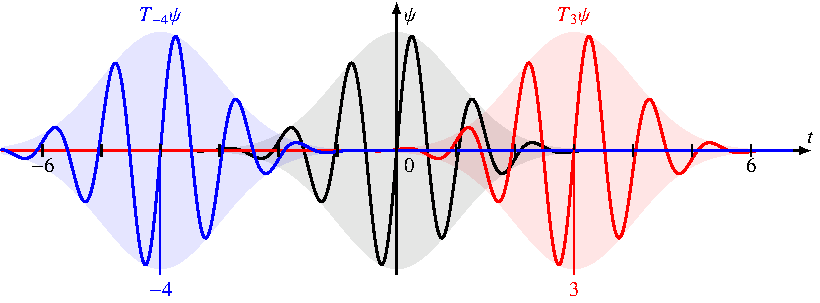
\includegraphics[width=\hsize]{chapters/1-geometrie/images/translation.pdf}
\caption{Wirkung des Operators $T_b$ auf das Gabor-Wavelet
$\psi(t) = e^{-t^2/2}\sin(6t)$,
der Graph von $T_b\psi$ ist um $b$ nach rechts verschoben.
\label{geometrie:Tb:image}}
\end{figure}
\begin{figure}
\centering
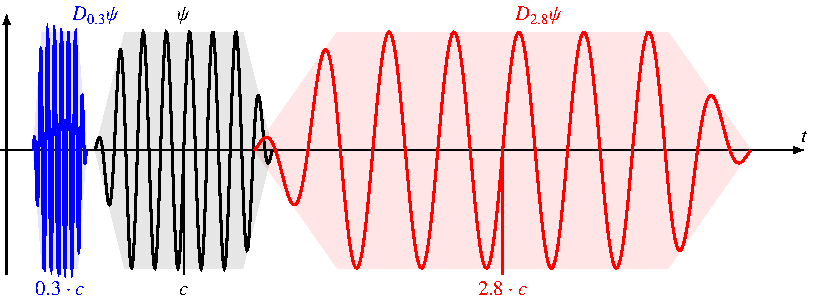
\includegraphics[width=\hsize]{chapters/1-geometrie/images/dilatation.pdf}
\caption{Wirkung des Operators $\tilde{D}_a$ auf ein im Punkt $c$ zentriertes
Wavelet $\psi$. Das Wavelet $\tilde{D}_a\psi$ ist zentriert im Punkt $a\cdot c$.
\label{geometrie:Da:image}}
\end{figure}

\begin{definition}
Sei $f$ eine Funktion auf $\mathbb R$ mit Werten in $Y$.
Dann setzt man
\begin{align*}
T_bf&\colon \mathbb R \to Y: t\mapsto f(t-b)&&\text{Translation}
\\
\tilde{D}_af&\colon \mathbb R \to Y: t\mapsto f(t/a)&&\text{Dilatation}
\end{align*}
\end{definition}

Die Wirkung der beiden Operatoren ist in den
Abbildungen~\ref{geometrie:Tb:image} und \ref{geometrie:Da:image} dargestellt.
Der Operator $\tilde{D}_a$ dehnt den Graphen der Funktion entlang der
$t$-Achse um den Faktor $a$ während der Operator $T_b$ den Graphen
der Funktion um den Betrag $b$ entlang der $t$-Achse verschiebt.

Die gewählte Notation für die Dilatation ist etwas asymmetrisch.
Der Grund ist, dass Operation $T_b$ die später zu definierende,
skalarproduktbasierte Norm erhält, dass aber $\tilde{D}_a$ diese Norm
verändert.
Die später formulierte Definition von $D_a$ wird erreichen, dass 
die $D_a$ die zum Skalarprodukt gehörige Norm erhält.

\begin{satz}
\label{geometrie:satz:inverse}
Die Operatoren $T_b$ und $\tilde{D}_a$ sind invertierbar und es gilt
\[
T_b^{-1} = T_{-b}
\qquad\text{und}\qquad
\tilde{D}_a^{-1} = \tilde{D}_{1/a}.
\]
\end{satz}

\begin{proof}[Beweis]
Die folgenden Rechnungen zeigen, dass $T_bT_{-b}f=f$ und $\tilde{D}_a\tilde{D}_{1/a}f=f$:
\begin{align*}
(T_bT_{-b}f)(t)
&=
(T_{-b})f(t-b)
=
f((t+b)-b)
=
f(t)
\\
(\tilde{D}_a\tilde{D}_{1/a}f)(t)
&=
(\tilde{D}_{1/a}f)(t/a)
=
f((t/{\textstyle\frac1a})/a)
=
f(t).
\qedhere
\end{align*}
\end{proof}

\begin{figure}
\centering
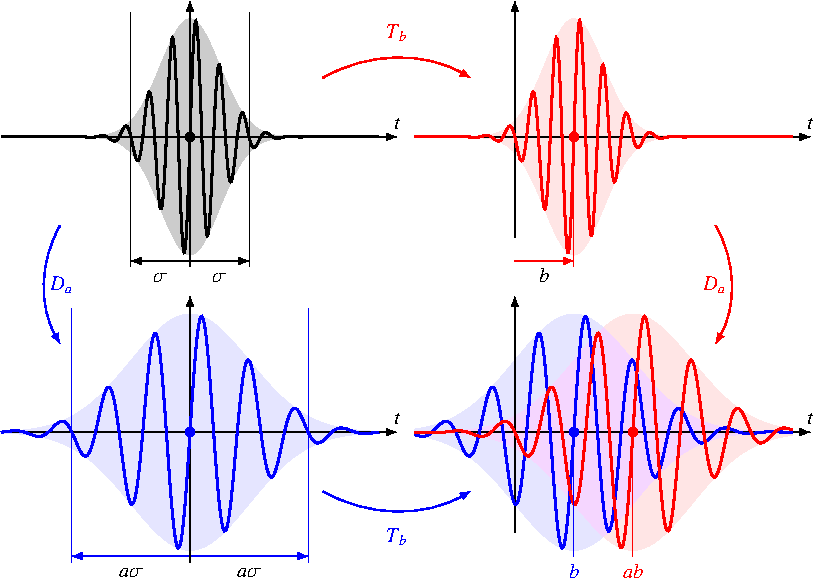
\includegraphics[width=\hsize]{chapters/1-geometrie/images/kommutator.pdf}
\caption{Die Operatoren $T_b$ und $D_a$ vertauschen nicht.
Der rote Pfad wendet erst $T_b$ und dann $D_a$ an, der blaue zuerst
$D_a$ und dann erst $T_b$.
In beiden Fällen erhält man ein um den Faktor $a$ gestrecktes
Wellenpaket.
Im Fall $T_b\circ D_a$ erhält man ein im Punkt $b$ zentriertes Wellenpaket
(blaue), während es im Falle $D_a\circ T_b$ im Punkt $ab$ zentriert ist (rot).
Wendet man in der unteren Zeile statt $T_b$ den Operator $T_{ab}$ an, 
kommen die beiden Wellenpakete zur Deckung, was die Vertauschungsregel
von Satz~\ref{satz:kommutator} bestätigt.
\label{geometrie:kommutator:image}}
\end{figure}

\begin{satz}
\label{satz:kommutator}
Translation $T_b$ und Dilatation $\tilde{D}_a$ sind lineare Abbildungen.
Die beiden Operatoren vertauschen nicht, vielmehr gilt
$T_{ab}\tilde{D}_a = \tilde{D}_aT_b$.
\end{satz}
\index{Vertauschungsregel für $T_b$ und $D_a$}%

\begin{proof}[Beweis]
Die Linearität der Operatoren wird durch Nachrechnen verifiziert.
Für eine Linearkombination $\lambda f+\mu g$ zweier Funktionen $f$ und $g$ gilt:
\begin{align*}
\tilde{D}_a(\lambda f+\mu g)(t)
&=
(\lambda f+\mu g)(t/a)
=
\lambda f(t/a)+\mu g(t/a)
=
\lambda (\tilde{D}_af)(t)+\mu (\tilde{D}_ag)(t),
\\
T_b(\lambda f+ \mu g)(t)
&=
(\lambda f+\mu g)(t-b)
=
\lambda f(t-b)+\mu g(t-b)
=
\lambda (T_bf)(t)+\mu (T_bg)(t).
\end{align*}
Ohne Argumente geschrieben heisst dies
\begin{align*}
\tilde{D}_a(\lambda f+\mu g) &= \lambda \tilde{D}_af + \mu \tilde{D}_ag,
\\
T_b(\lambda f+\mu g) &= \lambda T_bf + \mu T_bg.
\end{align*}
Damit ist die Linearität bewiesen.

Für die Vertauschungsregel müssen die beiden Seiten der Regel
berechnet werden.
Die Wirkung der beiden Operatoren in verschiedener Reihenfolge
ist:
\begin{align*}
(T_bf)(t)
&=
f(t-b),
\\
(\tilde{D}_af)(t)
&=
f(t/a),
\\
(\tilde{D}_aT_bf)(t)
&=
(T_bf)(t/a)
=
f(t/a-b)
=
f((t-ab)/a),
\\
(T_{ab}\tilde{D}_a f)(t)
&=
(\tilde{D}_af)(t - ab)
=
f((t-ab)/a).
\end{align*}
Daraus kann man ablesen, dass $T_{ab}\tilde{D}_a=\tilde{D}_aT_b$ ist.
\end{proof}

Die Abbildung~\ref{geometrie:kommutator:image} illustriert die
Vertauschungsregel für die Operatoren $T_b$ und $\tilde{D}_a$ und liefert
einen ``graphischen'' Beweis für die Vertauschungsregel von
Satz~\ref{satz:kommutator}.


%
% hilbertraum.tex
%
% (c) 2019 Prof Dr Andreas Müller, Hochschule Rapperswil
%
\section{Hilbertraum
\label{section:hilbertraum}}
\rhead{Hilbertraum}
Die bisher entwickelte Theorie ist aus zwei Gründen nicht ausreichend für das,
was wir vorhaben.

Ein endlichdimensionaler Vektorraum ist sicher ein geeigneter Rahmen zur
Beschreibung eines Signals, welches an endlich vielen Stellen abgetastet
wurde.
Für kontinuirliche Signale reicht er aber nicht.
Zunächst ist die Menge aller Funktionen zwar ein Vektorraum, aber es ist
aussichtslos, eine endliche orthonrmierte Basis zu finden.
Vielmehr werden wir sehen, dass bereits der Raum der stetigen Funktionen
auf einem Interval unendlich viele Funktionen enthält, die in einem noch
zu definierenden Sinn aufeinander senkrecht stehen.
Wir müssen daher den Begriff erweitern, so dass auch unendlichdimensionale
Vektorräume behandelt werden können.

In der Praxis tauchen nicht nur Signale mit rellen Werten auf, sondern
auch solche mit komplexen Werten.
An entscheidenden Stellen im vorangegangen Abschnitt, insbesondere bei
der Konstruktion der Norm, haben wir verwendet,
dass $x^2\le 0$ ist für $x\in\mathbb R$. Für $x\in\mathbb C$ ist dies
nicht mehr wahr.
Der bisher formulierte Begriff des Skalarproduktes funktioniert daher
nicht für komplexe Signale.

\subsection{Komplexe Vektorräume mit Skalarprodukt}
Es hindert uns nichts daran, in der Definition eines Vektorraums für die
Menge der Skalare auch komplexe Zahlen zuzulassen.
Ganz allgemein kann ein Vektorraum sinnvoll definiert werden, wenn die Menge
der Skalare ein sogenannter Körper ist, wenn also die Addition
und die Multiplikation mit von $0$ verschiedenen Skalaren umkehrbar ist.
Dies trifft natürlich für komplexe Zahlen zu, aber auch für $\mathbb Q$.

Die Definition der Länge eines Vektors und des Skalarproduktes auf dem
Vektorraum $\mathbb C^n$ erfordert aber etwas mehr Sorgfalt.
Die Quadratsumme der Komponenten funktioniert sicher nicht, da komplexe
Zahlen negative Quadrate haben können.
Die naheliegende Norm ist daher
\begin{equation}
\|v\| = \sum_{k=1}^n |v_k|^2.
\label{buch:hilbert:norm1}
\end{equation}
Sie ist für alle von $0$ verschiedenen Vektoren positiv, also positiv
definit.
Wir wollen diese Norm aber aus einem Skalarprodukt gewinnen.
Eine Möglichkeit ist
\begin{equation}
\langle u,v\rangle = \sum_{k=1}^n u_k\bar{v}_k.
\label{hilbert:skalaransatz}
\end{equation}
Die zugehörige Norm ist \eqref{buch:hilbert:norm1}.

Allerdings ist diese Bildung nicht mehr linear im zweiten Faktor.
Multipliziert man $v$ mit $\lambda$ erhält man
\[
\langle u,\lambda v\rangle
=
\sum_{k=1}^n u_k\bar{\lambda} \bar{v}_k
=
\bar{\lambda}\sum_{k=1}^n u_k\bar{v}_k
=
\bar{\lambda}\langle u,v\rangle.
\]
Man sagt, $\langle\;,\;\rangle$ ist {\em konjugiert linear} im zweiten Argument.
Im ersten Argument ist $\langle\;,\;\rangle$ aber immer noch linear.

Die Konstruktion~\eqref{hilvert:skalaransatz} ist auch nicht mehr
symmetrisch, vielmehr gilt:
\[
\langle v,u\rangle
=
\sum_{k=1}^n v_k\bar{u}_k
=
\overline{\sum_{k=1}^n u_k\bar{v}_k}
=
\overline{\langle u,v\rangle}.
\]
Vertauschen der Faktoren führt zum konjugiert komplexen Wert des
Skalarproduktes.
Man nennt diese Symmetrieeigenschaft von $\langle\;,\;\rangle$
{\em hermitesch}.
Hermitesche Formen zeichnen sich dadurch aus, dass
\[
\overline{\langle {\color{red}u},{\color{blue}u}\rangle}
=
\langle {\color{blue}u},{\color{red}u}\rangle.
\]
Nur die reellen Zahlen sind zu sich selbst konjugiert komplex, man kann
also schliessen, dass für eine hermitesche Form
$\langle u,u\rangle\in\mathbb R$ ist.

Dies führt uns auf die folgende Definition eines Skalarproduktes für einen
komplexen Vektorraum.
\begin{definition}
Eine Funktion
\[
\langle\;,\;\rangle
\colon V\times V\to \mathbb C : (u,v) \mapsto \langle u,v\rangle
\]
heisst ein komplexes Skalarprodukt, wenn gilt:
\begin{enumerate}
\item $\langle \;,\;\rangle$ ist linear im ersten Argument.
\item $\langle \;,\;\rangle$ ist konjugiert linear im zweiten Argument.
\item $\langle\;,\;\rangle$ ist hermitesch,
d.~h.~$\langle u,v\rangle=\overline{\langle v,u\rangle}$.
\item $\langle \;,\;\rangle$ ist positiv definit, d.~h.~es gilt
$\langle u,u\rangle \ge 0$ mit Gleichheit nur falls $u=0$.
\end{enumerate}
\end{definition}

Die Herleitung der Cauchy-Schwarz-Ungleichung hat die Symmetrie
und die Bilinearität des Skalarproduktes verwendet, sie lässt sich
also auf diese hermitesche Skalarprodukt nicht direkt übertragen.

\begin{satz}
Sei $V$ ein komplexer Vektorraum mit komplexem Skalarprodukt
$\langle\;,\;\rangle$,
dann gilt
\[
|\langle u,v\rangle| \le \|u\|\cdot \|v\|
\]
mit Gleichheit genau dann, wenn $u$ und $v$ linear abhängig sind.
\end{satz}

\begin{proof}[Beweis]
Wie im reellen Fall berechnen wird die Norm von $u+tv$:
\begin{align*}
0&\le
\| u+tv\|=\langle u+tv,u+tv\rangle
=
\|u\|^2 + \bar{t}\langle u,v\rangle + t\langle v,u\rangle + |t|^2 \|v\|^2
\\
&=
\|u\|^2 + \bar{t}\langle u,v\rangle + t\overline{\langle u,v\rangle} + |t|^2 \|v\|^2
\end{align*}
mit Gleichheit genau dann, wenn $u+tv=0$.
Die mittleren beiden Terme enthalten das Skalarprodukt, durch die Wahl
$t=-\langle u,v\rangle/\|v\|^2$ wird daraus
\begin{align*}
0
&\le
\|u\|^2 - 2\frac{|\langle u,v\rangle|^2}{\|v\|^2}
+
\biggl(\frac{|\langle u,v\rangle|}{\|v\|^2}\biggr)^2\|v\|^2
\\
&=
\|u\|^2 - \frac{|\langle u,v\rangle|^2}{\|v\|^2}.
\end{align*}
Multiplikation mit $\|v\|^2$ liefert
\begin{align*}
0&\le \|u\|^2 \cdot \|v\|^2 - |\langle u,v\rangle|^2
\\
\Leftrightarrow
\qquad
|\langle u,v\rangle|^2
&\le \|u\|^2 \cdot \|v\|^2
\end{align*}
mit Gleichheit genau dann, wenn $u+tv=0$.
Damit ist die Cauchy-Schwarz-Ungleichung auch für den komplexen Fall bewiesen.
\end{proof}

Auch für ein komplexes Skalarprodukt gilt, dass die Werte der Norm
das Skalarprodukt eindeutig bestimmen.
Da die Norm jedoch immer reelle Werte annimmt, ist etwas mehr Arbeit
erforderlich, um den Imaginärteil des Skalarproduktes wiederzugewinnen.
Znächst rechnen wir wie im Fall des reellen Skalarproduktes
\begin{align*}
\| u+v\|^2 
&=
\|u\|^2 + \langle u,v\rangle + \langle v,u\rangle + \|v\|^2
\\
&=
\|u\|^2 + \langle u,v\rangle + \overline{\langle u,v\rangle} + \|v\|^2
\\
&=
\|u\|^2 + 2\operatorname{Re}\langle u,v\rangle + \|v\|^2
\\
\Rightarrow\qquad
\operatorname{Re}\langle u,v\rangle
&=
\frac12(
\|u+v\|^2 - \|u\|^2 - \|v\|^2
).
\intertext{
Um den Imaginärteil zu bekommen, multiplizieren wir $v$ mit $i$:
}
\|u+iv\|^2
&=
\|u\|^2 + \langle u,iv\rangle + \langle iv,u\rangle + \|iv\|^2
\\
&=
\|u\|^2 -i \langle u,v\rangle + i\langle v,u\rangle + |i|^2 \|v\|^2
\\
&=
\|u\|^2 + \|v\|^2
-i (\langle u,v\rangle - \overline{\langle u,v\rangle})
\\
&=
\|u\|^2 + \|v\|^2
-i (2i\operatorname{Im}\langle u,v\rangle)
\\
&=
\|u\|^2 + \|v\|^2
+ 2\operatorname{Im}\langle u,v\rangle
\\
\Rightarrow\qquad
\operatorname{Im}\langle u,v\rangle
&=
\frac12(
\|u+iv\|^2- \|u\|^2 - \|v\|^2)
\end{align*}
Zusammengesetzt finden wir die Formel
\begin{equation}
\langle u,v\rangle
=
\frac12(
\|u+v\|^2 - \|u\|^2 - \|v\|^2
)
+
\frac{i}2(
\|u+iv\|^2- \|u\|^2 - \|v\|^2)
)
\label{hilbert:polarisierung}
\end{equation}
für das Skalarprodukt zweier beliebiger Vektoren, ausgedrückt
ausschliesslich mit der Norm.
Die Identität \eqref{hilbert:polarisierung} ist auch bekannt unter dem
Namen Polar-Identität.

Das Skalarprodukt erlaubt auch in einem komplexen Hilbertraum den Begriff
der orthonormierten Basis zu definieren.

\begin{satz}
Wenn die Vektoren $\{e_k\,|\, 1\le k\le n\}$ eine orthonormierte Basis
von $V$ bilden, dann lässt sich jeder Vektor $v\in V$ als Linearkombination
\[
v
=
\sum_{k=1}^n \hat{v}_k e_k
\]
der Vektoren $e_k$ schreiben.
Die Koeffizienten sind eindeutig bestimmt und können mit Hilfe des
Skalarproduktes als
\[
\hat{v}_k = \langle v,e_k\rangle
\]
gefunden werden.
Ausserdem gilt für das Skalarprodukt die Parseval-Identität
\begin{align*}
\langle u,v\rangle &= \sum_{k=1}^n \hat{u}_k\bar{\hat{v}}_k
\\
\| u \|^2 &= \sum_{k=1}^n |\hat{u}_k|^2.
\end{align*}
\end{satz}

Die Abbildung $T\colon V\to \mathbb C^n: v\mapsto (\hat{v}_k\,|\,1\le k\le n)$
ist also wie im reellen Fall eine Isometrie.


\subsection{Norm und Grenzwert in einem Hilbertraum}
Bis jetzt haben wir immer in endlichdimensionalen Vektorräumen gearbeitet.
Der tiefere Grund dafür war, dass die Arbeit mit unendlich vielen Basisvektoren
$e_k$, $k\in\mathbb N$, erfordert, dass Ausdrücken der Form
\begin{equation}
\sum_{k=1}^\infty a_k e_k
\label{hilbert:summe}
\end{equation}
ein Sinn gegeben werden muss.
Die Algebra reicht dazu nicht, denn zum Ende der Berechnung einer Summe
ohne Ende kann man grundsätzlich nicht gelangen.
Ein Ausdruck wie \eqref{hilbert:summe} kann daher nur im Sinne eines
Grenzwertes verstanden werden.
In einem Vektorraum ist aber a priori nicht definiert, wie man die
Approximation eines Vektors $v$ durch eine Folge von Vektoren $v_k$ zu
verstehen hat.

Mit der Einführung des Skalarproduktes und der daraus abgeleiteten Norm
ändert sich das.
\begin{definition}
Sei $V$ ein Vektorraum mit Skalarprodukt.
Eine Folge $v_k\in V$ konvergiert gegen den Vektor $v\in V$ für $k\to\infty$,
wenn
\[
\| v_k - v\| \to  0 
\qquad\Leftrightarrow\qquad
\lim_{k\to\infty} v_k = v.
\]
\end{definition}

Man erwartet, dass eine Folge einen Grenzwert hat, wenn die Folgenglieder
immer näher zueinander rücken.

\begin{definition}
Eine Folge $v_k\in V$ heisst Cauchy-Folge, wenn es für jedes $\varepsilon > 0$
ein $N(\varepsilon)\in\mathbb N$ gibt, so dass
$\|v_k - v_m\| < \varepsilon$
sobald $k,m>N(\varepsilon)$.
\end{definition}

Leider ist nicht garantiert, dass in einem komplexen Vektorraum eine
Cauchy-Folge auch tatsächlich einen Grenzwert hat.

\begin{beispiel}
Wir betrachten den Vektorraum
\[
c_0 = \{ X=(x_0, x_1, \dots ,x_k,0,\dots)\,| x_i \in \mathbb C\}
\]
von Folgen, die nur endlich viele Terme haben, die von $0$ verschieden sind.
Wir können diesem Vektorraum ein Skalarprodukt verpassen, indem wir
\[
\langle X,Y\rangle
=
\sum_{k=1}^\infty x_k\bar{y}_k
\]
setzen.
Da in beiden Folgen nur endlich viele Terme von $0$ verschieden sind, ist
die Summe auf der rechten Seite eine endliche Summe.
Ganz offensichtlich ist dies ein komplexer Vektorraum mit Skalarprodukt.
Jetzt betrachten wir die Folge
\begin{align*}
X_1 &= (1,0,0,0,\dots)
\\
X_2 &= (1,\frac12,0,0,\dots)
\\
X_3 &= (1,\frac12,\frac13,0,\dots)
\\
&\vdots
\\
X_k &= (1,\frac12,\frac13,\dots,\frac1k,0,\dots)
\\
&\vdots
\end{align*}
Wir behaupten, dies sei ein Cauchy-Folge.
Dazu müssen wir Differentzen $\| X_n-X_m\|$ untersuchen.
Wir dürfen annehmen, dass $m < n$ ist.
Dann ist
\begin{equation}
\| X_n - X_m\|^2 = \sum_{k=m+1}^n \frac{1}{k^2}.
<
\sum_{k=m+1}^\infty \frac{1}{k^2}.
\label{hilbert:eulercauchy}
\end{equation}
Auf der rechten Seite steht ein Reststück der Reihe
\[
\sum_{k=1}^\infty \frac{1}{k^2},
\]
die Euler als erster berechnet hat.
Er hat den Wert $\frac{\pi^2}{6}$ gefunden.
Die Tatsache, dass die Reihe konvergiert heisst aber auch, dass
es für jedes $\varepsilon >0$ eine Zahl $N(\varepsilon)$ gibt derart,
dass die rechte Seite von \eqref{hilbert:eulercauchy} kleiner ist
als $\varepsilon$, wenn nur $m,n>N(\varepsilon)$.
Die Folge $(X_k)$ ist also tatsächlich ein Cauchy-Folge.

Als Grenzwert kommt nur die Folge 
\[
X = (1,\frac12, \frac13,\frac14,\dots)
\]
in Frage.
Und tatsächlich ist
\begin{equation}
\|X-X_n\|^2
=
\sum_{k=n+1}^\infty \frac1{k^2},
\label{hilbert:falscherabstand}
\end{equation}
wieder ein Reststück der Reihe von Euler.
Also konvergiert tatsächlich $X_k$ gegen $X$.

Die Folge $X$ ist aber gar nicht in $c_0$,
da alle Folgenglieder von $0$ verschieden sind.
Der Grenzwert einer Folge in $c_0$ muss also nicht mehr in $c_0$ sein.

Genau genommen haben wir schon in \eqref{hilbert:falscherabstand}
gemogelt.
Die Abstandsmessung in $c_0$ ist ja mit Hilfe einer endlichen Summe
definiert, hier haben wir aber eine unendliche Summe.
\end{beispiel}

Die Rekonstruktion eines Vektors mit Hilfe einer Linearkombination von
Basisvektoren kann also grundsätzlich nur dann funktionieren, wenn verlangt
wird, dass es zu jeder Cauchy-Folge von Vektoren auch tatsächlich einen
Grenzwert gibt.

\begin{definition}
Ein komplexer Vektorraum $V$ mit Skalarprodukt heisst {\em vollständig}, 
wenn jede Cauchy-Folge von Vektoren in $V$ einen Grenzwert in $V$ hat.
Ein solcher Vektorraum heisst {\em Hilbertraum}.
\end{definition}

Der Vektorraum $c_0$ des obigen Beispiels lässt sich leicht zu einem
Hilbertraum machen.

\begin{beispiel}
Sei $l^2$ der komplexe Vektorraum der quadratsummierbaren komplexen
Zahlfolgen $(x_k)$, d.~h.
\[
l^2 = \left\{ (x_k)\,\left| \sum_{k=1}^\infty |x_k|^2 < \infty \right.\right\}
\]
mit dem Skalarprodukt
\[
\langle X,Y\rangle = \sum_{k=1}^\infty x_k\bar{y}_k.
\]
% XXX TODO: Vervollständigung: Summierbarkeit des Grenzwertes...
\end{beispiel}

\subsection{Basis eines Hilbertraumes}



